\chapter{Methodology}

\section{Rendered Datasets}

We find ourselves in the situation where we want to train a 6D pose estimation model on a certain set of objects, that are not present in any available dataset. This necessarily means that we must create our own datasets for training and evaluation.

To create our own datasets we require images with their associated ground truths. However, collecting this data in the real world is tedious and difficult, considering that any errors or biases will affect the perfomance of the final model. 

One possible solution is to use rendering software, which can generate potentially infinite quantites of training images. However, while a model trained on this data could certainly work well in simulation, we have no guarantee whether it would also function with real life images. This is because a simulated sensor and simulated enviroment are unable to reproduce unmodeled physical effects and noise in the same way an optical sensor would. This issue is dubbed the "reality gap"\cite{domainRandomization2}, and there are various ways we could attempt to solve it.

\subsection{Randomized Domain Dataset}

Domain Randomization\cite{domainRandomization} is the most readily available method for bridging the reality gap. The hypothesis behind this concept states that introducing sufficient variability in the simulated training domain will allow the model to generalise to the real world with no additional steps. In our situation, the domain is an image, so we have huge liberty in choosing how to randomize it.

For our first attempt, we decided to generate a dataset for estimating the pose of a single object: a standard M6x30 hexagonal head screw. This is a very challenging object for pose estimation, as it is small (34 mm in length) and symmetric. The reason why symmetric objects are difficult for pose estimation is explained in depth in section (t.b.a.).

To render the images in our dataset, we use Unity's Perception package\cite{unityPerception}, which integrates domain randomization features into its pipeline. Unity Perception works by implementing an object called a scenario, which is connected to a set of scripts called randomizers. When we run a scenario, we specify the number of iterations and the number of frames we want to render for each iteration, and at the beginning of each iteration, all randomizers connected to the scenario are called to set one of the domain variables. These variables can be anything within the scene, from positions and rotations of objects to textures and colors.

\begin{figure}
    \centering
    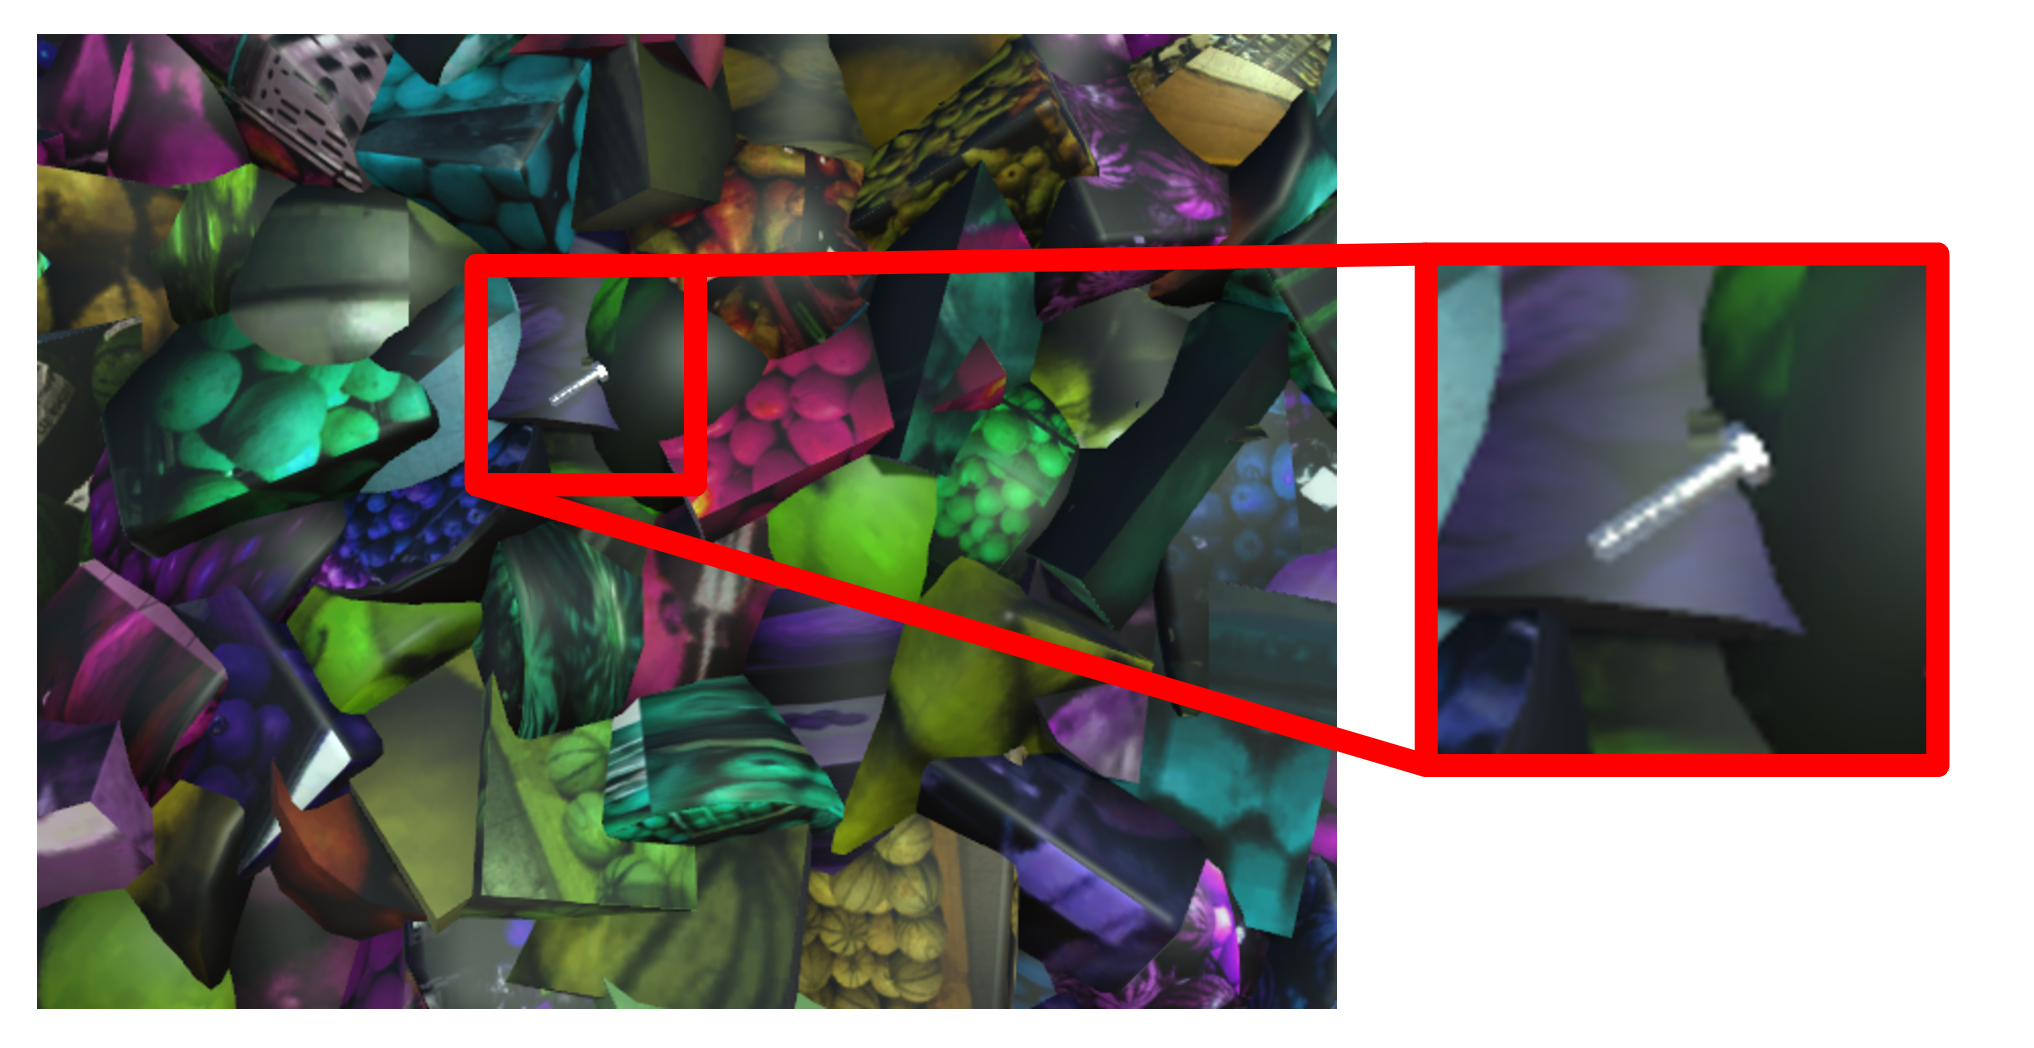
\includegraphics[width=0.6\textwidth]{screwdataset/ScrewDataset.png}
    \caption{One of the images generated with Unity's Perception package for training our model, with a zoom-in on the screw.}
    \label{fig:screwdataset}
\end{figure}

For our dataset, we implemented a scenario with 10'000 iterations lasting one frame each. We used a model of the M6x30 screw obtained from the FreeCAD Fasteners workbench\cite{Fasteners}, and then used a custom randomizer to set its position and rotation for each iteration. We then used default randomizers provided as samples by Unity as part of its Perception package to generate a background, composed by random shapes placed with random positions, orientations and textures. Finally, we used a custom randomizer to set the lighting color, intensity and origin. A sample image from this dataset appears in figure \ref{fig:screwdataset}.

We then converted the Unity output to a format that we could feed to EfficientPose for training. This required converting the ground truths from Unity's internal left-handed reference system to the right-handed reference used by the rest of the world, and generating other relevant information required by EfficientPose, such as mask information and the dimensions, center and diameter of the 3D bounding box enveloping the model of the screw.